\chapter{A brief theory of Markov chains}
\label{chap:markov}

\section{Markov chains}
We conduct an experiment with a set of $r$ \emph{outcomes} or \emph{states},
\[
S=\{S_1,\dots, S_r\}.
\]
The experiment is repeated $n$ times (with $n$ large, potentially infinite). 
The system has no memory: the next state depends only on the present state. 
The probability of $S_j$ occurring on the next step, given that $S_i$ occurred on the last step, is
\[
p_{ij}=p(S_j|S_i).
\]
Suppose that $S_i$ is the current state, then one of $S_1, \ldots,S_r$ must be the next state; therefore,
\[
p_{i1}+p_{i2}+\cdots+p_{ir}=1, \quad 1\leq i\leq r.
\]
(Note that some of the $p_{ij}$ can be zero, all that is needed is that $\sum_{j=1}^r p_{ij}=1$ for all $i$.)

\begin{definition}
An experiment with finite number of possible outcomes $S_1,\ldots,S_r$ is repeated. The sequence of outcomes is a \emph{Markov chain} if there is a set of $r^2$ numbers $\{p_{ij}\}$ such that the conditional probability of outcome $S_j$ on any experiment given outcome $S_i$ on the previous experiment is $p_{ij}$, i.e., for $1\leq i,j\leq r$, $n=1,\ldots$,
\[
p_{ij}=\mathsf{Pr}(S_j\textrm{ on experiment }n+1|S_i\textrm{ on experiment }n).
\]
The outcomes $S_1,\ldots,S_r$ are the \emph{states}, and the $p_{ij}$ are the \emph{transition probabilities}. The matrix $P=[p_{ij}]$,
\[
P=
\begin{pmatrix}
p_{11} & p_{12} & \cdots & p_{1r} \\
p_{21} & p_{22} & \cdots & p_{2r} \\
&&& \\
p_{r1} & p_{r2} & \cdots & p_{rr}
\end{pmatrix},
\]
is called the \emph{transition matrix} of the Markov chain. 
\end{definition}
The transition matrix has
\begin{itemize}
\item nonnegative entries, $p_{ij}\geq 0$
\item entries less than 1, $p_{ij}\leq 1$
\item row sum equal to 1, which we write
\[
\sum_{j=1}^r p_{ij}=1,\quad i=1,\ldots,r
\]
or, using the notation $\nbOne^T=(1,\ldots,1)$,
\[
P\nbOne=\nbOne.
\]
\end{itemize}
These properties guarantee that the elements of the matrix $P$ describe probabilities.


\section{Repetition of the process}

Let $p_i(n)$ be the probability that the state $S_i$ will occur on the $n^{th}$ repetition of the experiment, $1\leq i\leq r$. 
Since one the states $S_i$ must occur on the $n^{th}$ repetition,
\[
p_1(n)+p_2(n)+\cdots+p_r(n)=1.
\]
Let $p_i(n+1)$ be the probability that state $S_i$, $1\leq i\leq r$, occurs on $(n+1)^{th}$ repetition of the experiment. 
There are $r$ ways to be in state $S_i$ at step $n+1$:
\begin{enumerate}
\item[1.] Step $n$ is $S_1$. Probability of getting $S_1$ on $n^{th}$ step is $p_1(n)$, and probability of having $S_i$ after $S_1$ is $p_{1i}$. Therefore, $P(S_i|S_1)=p_{1i}p_1(n)$. 
\item[2.] We get $S_2$ on step $n$ and $S_i$ on step $(n+1)$. Then $P(S_i|S_2)=p_{2i}p_2(n)$. 
\item[..]
\item[r.] Probability of occurrence of $S_i$ at step $n+1$ if $S_r$ at step $n$ is $P(S_i|S_r)=p_{ri}p_r(n)$.
\end{enumerate}
Therefore, $p_i(n+1)$ is sum of all these probabilities,
\begin{align*}
p_i(n+1) &= P(S_i|S_1)+\cdots+P(S_i|S_r) \\
&= p_{1i}p_1(n)+\cdots+p_{ri}p_r(n)
\end{align*}
Therefore,
\begin{equation}\label{eq:chain1}
\begin{aligned}
p_1(n+1) &= p_{11}p_1(n)+p_{21}p_2(n)+\dots+p_{r1}p_r(n) \\
& \vdots\\
p_k(n+1) &= p_{1k}p_1(n)+p_{2k}p_2(n)+\dots+p_{rk}p_r(n) \\
& \vdots\\
p_r(n+1) &= p_{1r}p_1(n)+p_{2r}p_2(n)+\dots+p_{rr}p_r(n)
\end{aligned}
\end{equation}
In matrix form
\begin{equation}
p(n+1)=p(n)P, \quad n=1,2,3,\dots
\end{equation}
where $p(n)=(p_1(n),p_{2}(n),\dots , p_r(n))$ is a (row) probability vector and $P=(p_{ij})$ is a $r\times r$ \emph{transition matrix},
\[
P=
\begin{pmatrix}
p_{11} & p_{12} & \cdots & p_{1r} \\
p_{21} & p_{22} & \cdots & p_{2r} \\
&&& \\
p_{r1} & p_{r2} & \cdots & p_{rr}
\end{pmatrix}
\]
So, what we have is
\[
(p_1(n+1),\ldots,p_r(n+1))=
(p_1(n),\ldots,p_r(n))
\begin{pmatrix}
p_{11} & p_{12} & \cdots & p_{1r} \\
p_{21} & p_{22} & \cdots & p_{2r} \\
&&& \\
p_{r1} & p_{r2} & \cdots & p_{rr}
\end{pmatrix}
\]
It is easy to check that this gives the same expression as \eqref{eq:chain1}.

\subsection{Long time behaviour}
Let $p(0)$ be the initial distribution (row) vector. Then
\begin{align*}
p(1) &= p(0)P \\
p(2) &= p(1)P\\
&= (p(0)P)P \\
&= p(0)P^2
\end{align*}
Iterating, we get that for any $n$,
\[
p(n)=p(0)P^n
\]
Therefore, 
\begin{equation}\label{eq:limit_Markov_chain}
\lim_{n\rightarrow +\infty}p(n)=\lim_{n\rightarrow +\infty}p(0)P^n=p(0)\lim_{n\rightarrow +\infty}P^n.
\end{equation}
So, to determine the long time behaviour of the Markov chain, it suffices to determine the limit of the $P^n$.


\subsection{Stochastic matrices}
One fundamental property of Markov chains is that the transition matrix $P$ has a very particular structure.
\begin{definition}[Stochastic matrix]
The nonnegative $r\times r$ matrix $M$ is a \emph{stochastic} matrix if $\sum_{j=1}^ra_{ij}=1$ for all $i=1,2,\dots, r$, i.e., the rows of $M$ all sum to 1.
\end{definition}
Note that a matrix that has column sums all equal to 1 is also called a stochastic matrix. Such a matrix arises if instead of representing transitions from rows to columns as we have done, transitions are represented from columns to rows. 
If it is needed to distinguish between matrices that are stochastic by rows or by columns, we say that, say, a matrix is a (row) stochastic matrix.

A matrix that that both rows and column sums equal to 1 is a \emph{doubly stochastic} matrix.
Stochastic matrices over $\IR_+$ form a \emph{group}. This means in particular that the following holds true.
\begin{theorem}
If $M,N$ are stochastic matrices, then $MN$ is a stochastic matrix.
\end{theorem}
This is particularly interesting, as it means that powers of a stochastic matrix are also stochastic:
\begin{theorem}
If $M$ is a stochastic matrix, then for any $k\in\IN$, $M^k$ is a stochastic matrix.
\end{theorem}
A stochastic matrix has the property that all its eigenvalues are contained in the unit disk of $\IC$.
\begin{theorem}
Let $M$ be a stochastic matrix $M$. Then the following two properties hold.
\begin{enumerate}
\item The \emph{spectral radius} of $M$, $\rho(M)$, is such that $\rho(M)=1$. In other words, all eigenvalues $\lambda$ of $M$ are such that $|\lambda|\leq 1$. Furthermore, $\lambda =1$ is an eigenvalue of $M$.
\item If $M$ is stochastic by rows, then $\lambda=1$ is associated to the eigenvector $\nbOne$, while if $M$ is stochastic by columns, then $\lambda=1$ is associated to the left eigenvector $\nbOne^T$.
\end{enumerate}
\end{theorem}
\begin{proof}
To see that $1$ is an eigenvalue, write the definition of a stochastic matrix, i.e., $M$ has row sums 1. In vector form, $M\nbOne=\nbOne$. Now remember that $\lambda$ is an eigenvalue of $M$, with associated eigenvector $v$, iff $Mv=\lambda v$. So, in the expression $M\nbOne=\nbOne$, we read an eigenvector, $\nbOne$, and an eigenvalue, $1$.
\end{proof}






\section{Regular Markov chains}
\begin{definition}[Regular Markov chain]
A regular Markov chain is one in which $P^k$ is positive for some integer $k>0$, i.e., $P^k$ has only positive entries, no zero entries.
\end{definition}
In matrix theory, this property is called \emph{primitivity}.
\begin{definition}
A nonnegative matrix $M$ is primitive if, and only if, there is an integer $k>0$ such that $M^k$ is positive.
\end{definition}
Therefore, we have the following result.
\begin{theorem}
A Markov chain is regular if, and only if, the transition matrix $P$ is primitive.
\end{theorem}
Another way to check regularity will then be using a sufficient condition for primitivity, given here.
\begin{theorem}\label{th:strong_conn_implies_primitive}
A matrix $M$ is primitive if the associated connection graph is strongly connected, i.e., that there is a path between any pair $(i,j)$ of states, and that there is at least one positive entry on the diagonal of $M$.
\end{theorem}
This is checked directly on the digraph associated to the transition matrix, shown for our model in Figure~\ref{fig:Markov_graph1}. The digraph is here strongly connected, and as there are positive entries on the diagonal of the matrix (as evidenced by the self-connecting loops on all vertices), the transition matrix associated to this graph is primitive, from Theorem~\ref{th:strong_conn_implies_primitive}.



\begin{theorem}
\label{th:limit_Markov_regular}
If $P$ is the transition matrix of a regular Markov chain, then
\begin{enumerate}
\item the powers $P^n$ approach a stochastic matrix $W$,
\item each row of $W$ is the same (row) vector $w=(w_1,\ldots,w_r)$,
\item the components of $w$ are positive.
\end{enumerate}
\end{theorem}
So if the Markov chain is regular,
\begin{equation}\label{eq:limit_Markov_regular}
\lim_{n\rightarrow +\infty}p(n)=p(0)\lim_{n\rightarrow +\infty}P^n
=p(0)W.
\end{equation}



\paragraph{Application to Markov chains}
We already know that the (right) eigenvector corresponding to the eigenvalue 1 is $\nbOne$.
The vector $w$ in Theorem~\ref{th:limit_Markov_regular} is in fact the left eigenvector corresponding to the eigenvalue 1 of $P$.
To see this, remark that, if $p(n)$ converges, then $p(n+1)=p(n)P$, so $w$ is a fixed point of the system. We thus write
\[
wP=w
\]
and solve for $w$, which amounts to finding $w$ as the left eigenvector corresponding to the eigenvalue 1.
\vskip0.5cm
Alternatively, we can find $w$ as the (right) eigenvector associated to the eigenvalue 1 for the transpose of $P$,
\[
P^Tw^T=w^T
\]
Now remember that when you compute an eigenvector, you get a result that is the eigenvector, to a multiple.
So the expression you obtain for $w$ might have to be normalized (you want a probability vector). Once you obtain $w$, check that the norm $\|w\|$ defined by
\[
\|w\|=w_1+\cdots+w_r
\]
is equal to one. If not, use
\[
\frac{w}{\|w\|}.
\]







\begin{definition}
A state $S_i$ in a Markov chain is \emph{absorbing} if whenever it occurs on the $n^{th}$ generation of the experiment, it then occurs on every subsequent step. In other words, $S_i$ is absorbing if $p_{ii}=1$ and $p_{ij}=0$ for $i\neq j$. A state that is not absorbing is called \emph{transient}.
\end{definition}

\begin{definition}
A Markov chain is said to be absorbing if it has at least one absorbing state, and if from every state it is possible to go to an absorbing state.
\end{definition}


Suppose we have a chain like the following:
\begin{center}
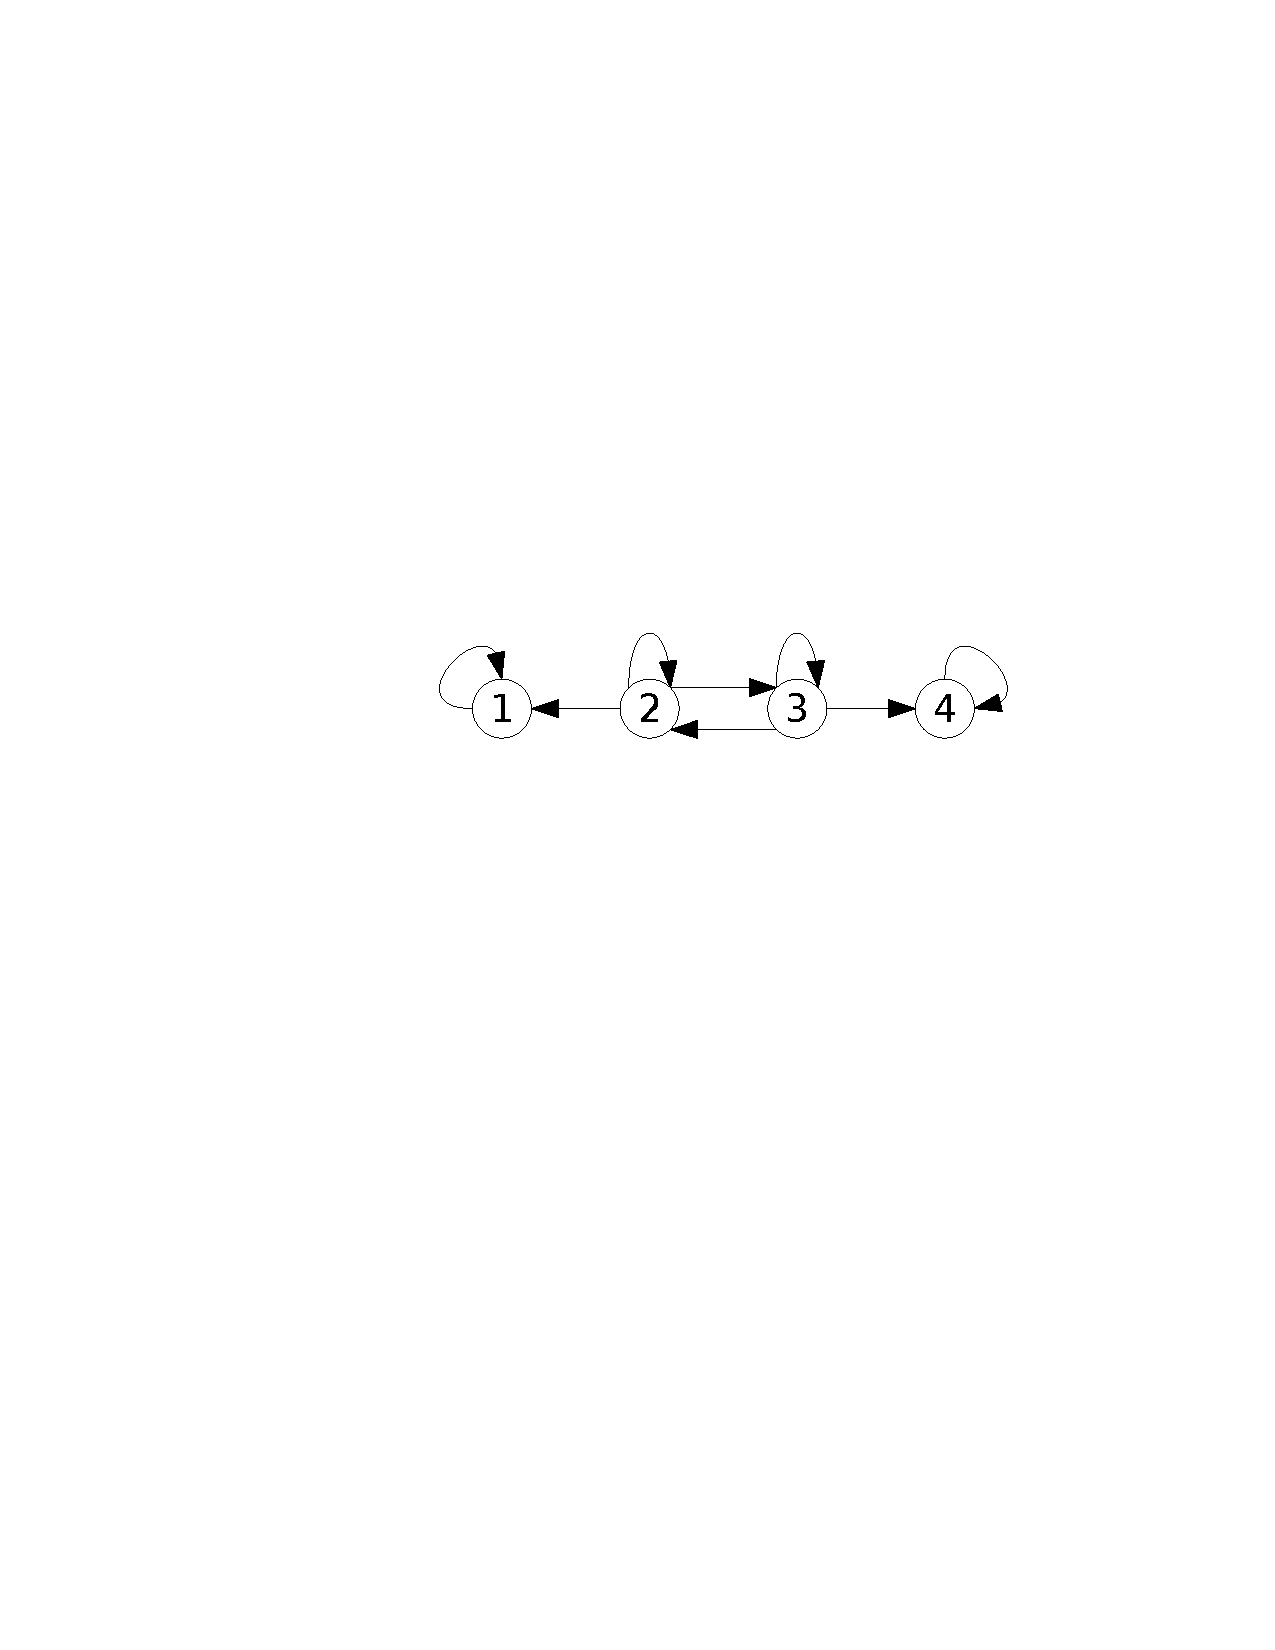
\includegraphics[width=0.45\textwidth]{../figs_08_genetics/graphe_absorbant}
\end{center}
\begin{enumerate}
\item Does the process eventually reach an absorbing state?
\item Average number of times spent in a transient state, if starting in a transient state?
\item Average number of steps before entering an absorbing state?
\item Probability of being absorbed by a given absorbing state, when there are more than one, when starting in a given transient state?
\end{enumerate}

Answer to question 1:
\begin{theorem}
In an absorbing Markov chain, the probability of reaching an absorbing state is 1.
\end{theorem}

For an absorbing chain with $k$ absorbing states and $r-k$ transient states, the transition matrix can be written in the following \textbf{standard form}:
\[
P=\begin{pmatrix}
\mathbb{I}_k & \mathbf{0} \\
R & Q
\end{pmatrix}
\]
with following meaning,
\begin{center}
\begin{tabular}{ccc}
& Absorbing states & Transient states \\
Absorbing states & $\mathbb{I}_k$ & $\mathbf{0}$ \\
Transient states & $R$ & $Q$
\end{tabular}
\end{center}
with $\mathbb{I}_k$ the $k\times k$ identity matrix, $\mathbf{0}$ an $k\times(r-k)$ matrix of zeros, $R$ an $(r-k)\times k$ matrix and $Q$ an $(r-k)\times(r-k)$ matrix.


The matrix $\mathbb{I}_{r-k}-Q$ is invertible. Let
\begin{itemize}
\item $N=(\mathbb{I}_{r-k}-Q)^{-1}$ be the \emph{fundamental matrix} of the Markov chain
\item $T_i$ be the sum of the entries on row $i$ of $N$
\item $B=NR$.
\end{itemize}
\vskip0.5cm
Answers to our remaining questions:
\begin{enumerate}
\setcounter{enumi}{1}
\item $N_{ij}$ is the average number of times the process is in the $j$th transient state if it starts in the $i$th transient state.
\item $T_i$ is the average number of steps before the process enters an absorbing state if it starts in the $i$th transient state.
\item $B_{ij}$ is the probability of eventually entering the $j$th absorbing state if the process starts in the $i$th transient state.
\end{enumerate}











\begin{definition}
A regular Markov chain is one in which $S^p$ is positive for some positive integer $p$.
\end{definition}

From Theorem \ref{Theo:NormRho}
$$\rho(S)\leq \| S\| _1 =1$$
then $|\lambda|\leq 1$ for all eigenvalues of a stochastic matrix. Furthermore, if $S$ is a stochastic matrix $\lambda =1$ is an eigenvalue of $S$; hence $\rho(S)=1$ and the dominant eigenvalue $\lambda _1 =1$. Then
$$\lim_{n\rightarrow +\infty}p(n)=\lim_{n\rightarrow +\infty}S^np(0)=cV_1$$
where $V_1=(v_1,v_2,\dots ,v_k)$ is the eigenvector that corresponds to the dominant eigenvalue $\lambda _1 =1$.

Since $p(n)=(p_1(n),p_2(n),\dots , p_k(n))^T$, we have $\sum_{i=1}^k p_i(n)=1$, it follows that
$$cv_1+cv_2+\dots cv_k=1.$$
Therefore
$$c=\frac{1}{v_1+v_2+\dots+v_k}.$$


\begin{definition}
A state $s_i$ in a Markov chain is said to be absorbing if whenever it occurs on the $n^{th}$ generation of the experiment, it then occurs on every subsequent repetition. In other word, if for some $p_{ii}=1$ then $p_{ij}=0$ for $i\not =j$.
\end{definition}

\begin{definition}
A Markov chain is said to be absorbing if it has at least one absorbing state, and if from every state it is possible to go to an absorbing state.
\end{definition}

In an absorbing Markov chain, a state that is not absorbing is called transient.
